\section{Defining the Strategy}
    Answer two basic questions:
    \begin{enumerate}
        \item What do we want to get from this product?
        \item What do our user want from this product?
    \end{enumerate}
    \begin{figure}
        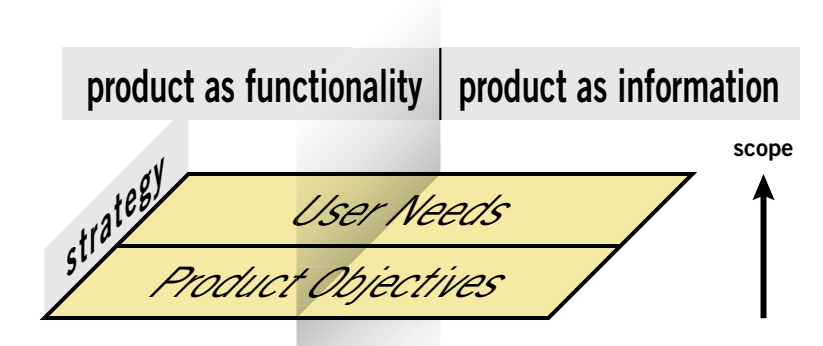
\includegraphics[width=\linewidth]{images/pic2.png}
        \caption{Strategy plane}
    \end{figure}
\section{Product Objectives}
    Is it a service or product? Usually we do not clear our objectives in case of product and thus different people will have different ideas.
\subsection{Business Goals}
    Sometimes you say, ‘To earn money’ or ‘To Save money’. These are too general. On the other hand, very specific, such as ‘To provide text messaging service for users’, which does not explain the requirement of you. We tell the conditions for success, not path.
\subsection{Brand Identity}
    Your brand is neither only a logo nor typography. It can be represented by users’ interaction with your website. This experience would be your brand.
\subsection{Success Metrics}
    You should have some concrete criterias which determines, when you have reached success. These are known as \textbf{success metrics}. These metrics may be :
    \begin{itemize}
        \item The average time, a user spends on the site
        \item Number of visits per registered user
        \item The number of time, each ads is displayed.
        \item The number of calls to support team.
        \item Number of return visits
    \end{itemize}
    Sometimes these metrics are influenced by other factors, For example: Ineffective advertisements. This should be taken into account.
\section{User Needs}
\subsection{User Segmentation}
\subsection{Usability and User Research}
\subsection{Creating Personas}
\section{Team Roles and Process}
